\chapter{Software of the Vision Correction Display}

\section{Introduction to Algorithms}

Fu-Chun Huang et al. utilized light field technology to generate a sharp image beyond the display plane \cite{Huang:EECS-2013-206}. Peter Wu introduced the forward method and its optimizations. Another new algorithm we will introduce is the backward method. We will use the same definitions and symbols in chapter 4 of Wu's thesis for consistency.

\subsection{Projection and Prefiltering}

Each algorithm in this paper is divided up into two components: the projection relationship and prefiltering. The projection relationship is the mapping relationship from a point on the display to a point on the sensor or retina. The projection relationship depends on the experimental settings such as focal point, object focus, and object distance. Prefiltering is the step in which the content on the display is modified. Prefiltering takes in the projection relationship and the input image and produces a transformed output image.

\subsection{Symbols}

\begin{figure}[ht]
  \centering
  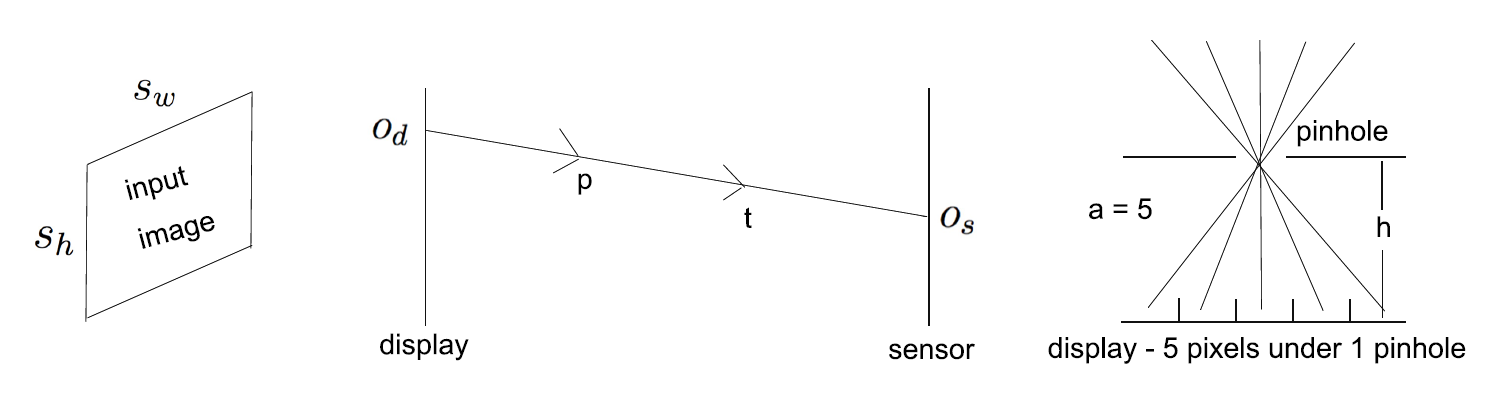
\includegraphics[width=5.0in]{chapters/chapter4/images/Prefilter.png}
  \caption{The figure shows the setup for the prefiltering algorithm. (left) The input image has dimensions $s_w$ by $s_h$ pixels. (middle) $p$ and $t$ are points on the light ray. (right) There are $5$ pixels under each pinhole, and $h$ is the distance between the pinhole and the display. This image is from [Wu 2016]}
  \label{fig:fr}
\end{figure}


The size of the input image is $s_w$ by $s_h$ pixels. The input image is the unmodified image a normal person sees on the display.
We define two functions $f_s$ and $f_d$, both of which contain the same parameters:
\begin{itemize}
\item $p$ and $t$ stand for arbitrary points in 3-D space. $p$ and $t$ specify a light ray.

\item $e$ is the experimental settings. If we only consider defocus (myopia or hyperopia) the only parameter to consider is the distance from the the screen to the lens.

\item $c$ is the condition of the camera or human eye. If we only consider defocus, then this parameter is the distance from the sensor to the lens.

\item
\end{itemize}

$f_s$ takes in the parameters and computes the position $o_d$, the position where the light ray $(p,t)$ hits the sensor. Similarly, $f_d$ takes in the same parameters and computes the position $o_s$, the position where the light ray $(p, t)$ hits the display. \\
$$f_s(p, t, e, c) \rightarrow O_s$$ \\
$$f_d(p, t, e, c) \rightarrow O_d$$ \\
The angular resolution $a$ is the ratio of the screen resolution to the pinhole mask display or lens array display. \\
The depth $h$ is the distance from the surface of the pinhole mask to the plane of the display.

\section{Huang's Light Field Algorithm}

The projection relation is represented as a matrix in Huang's algorithm. He assumes that the sensor has the same resolution as that of the pinhole mask, which is ($L_s = s_w / a$ by $L_d = s_h / a$). This display pixels have resolution $s_w$ $\times$ $s_h$. 
Next, the algorithm builds a projection matrix. First, an all-zero matrix $P$ with dimensions $L_d$ by $L_s$ is created. Second, for every pixel on the screen, n points $o_n$ are sampled on the aperture, and a light ray $p_s - o_i$ is constructed for each sample point. third, the algorithm applies the function $f_d$ to get the position $p_d$ on the display. Then, the function $m_d$ is called to convert $p_d$ into a 2-D index $I_d$. Finally, algorithms adds index $I_d$ of the matrix by $1/n$. 

After the projection matrix is formed, the following linear equation needs to be solved, where $P$ is the project matrix and $b$ is the one-dimensional representation of the input image:

$$P \cdot x = b$$

$P$ is not a square matrix, but we can multiply both sides by $P^{T}$, and $P^TP$ is square.

$$(P^T \cdot P) \cdot x = p^T \cdot b$$

Define $H = P^T \cdot P$. There is a high chance that $H$ is singular and there is not solution to the linear system. To solve the linear system, a very small positive value $\lambda$ is defined and added to the the system where $I$ is the identity matrix:

$$H' \leftarrow H + \lambda \cdot I$$

$\lambda$ introduces a negligible amount of error to the system, and $H$ is not singular anymore.

Instead of solving the system directly, Huang's algorithm changes it into an optimization problem: \\

Minimize: $$(H'x - P^Tb)^T \cdot (H'x-P^Tb)$$

the L-BGFS method was used to solve this optimization problem. The final result $x$ may have very large positive or very small negative values, but Huang cut off all values in the range (0, 255). The algorithm was applied for the R, G, and B (red, green, and blue) channels separately.


\section{Forward Method}

In the forward method, we assume that the sensor has the same resolution as the screen, so if the screen has size $640 \times 640$ pixels, then so does the sensor. In addition, the light rays travel from the screen to the sensor instead of from the sensor to the screen.

The first step in the algorithm is to the set the sensor image equal to the original perfect image. For each display pixel $p_d$, a ray is drawn from the center of $p_d$ to the center position of the closest pinhole, $o_c$. That ray is then traced to the sensor, and the color on the sensor position $o_s$ is equal to the color on the display position $o_d$. 

\lstset {language=C++}
\begin{lstlisting}[frame=single, caption=Pseudocode For Prefiltering Algorithm]
int[][] sensor_image = origin_image;
int[][] prefiltered_image = new int[sensor_image.height][sensor_image.width];

// Loop through the display image
for (int y_index = 0; y_index < screen_size; y_index++) {
  for (int x_index = 0; x_index < screen_size; x_index++) {
        screen_pos = [x_index, y_index];
        pinhole_pos = find_nearest_pinhole(screen_pos);
        sensor_pos = ray_trace(screen_pos, pinhole_pos, sensor_image);
        prefiltered_image[x_index][y_index] = sensor_image[sensor_pos];
  }
}
\end{lstlisting}

Figure 5 shows the results of running the prefiltering algorithm on a clean image. Note that the black borders represent screen pixels that do not reach the sensor. The prefiltering algorithm is the same as the forward method described in \textit{Investigating Computational Approaches and Proposing Hardware Improvement to the Vision Correcting Display} [Wu 2016].

\begin{figure}[ht]
  \centering
  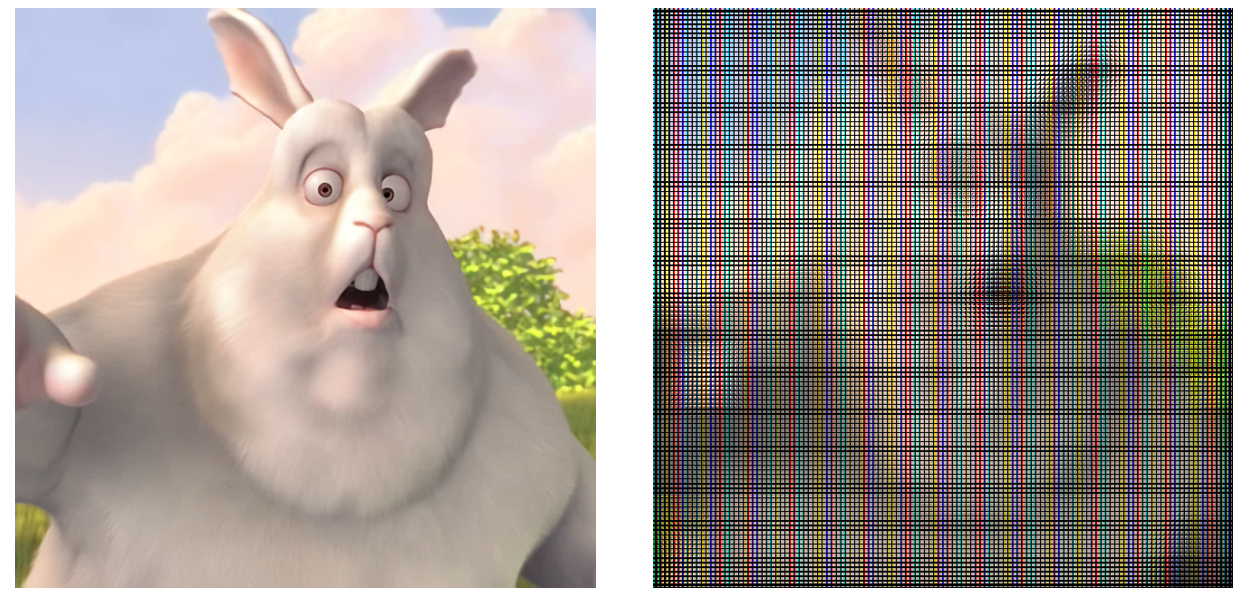
\includegraphics[width=3.5in]{chapters/chapter4/images/Original_Prefiltered.png}
  \caption{Original Image (left) and Prefiltered Image (right)}
  \label{fig:fr}
\end{figure}

\section{Backward Method}

In the backward method, rays are traced form the sensor to the screen, like in Huang's algorithm. We also assume that the resolution of the sensor and screen are the same. 

The first step in the algorithm is to the set the sensor image equal to the original perfect image and the display image equal to a $s_w \times s_h$ array of zeros. For each sensor pixel $o_d$, a ray is drawn to the center position of the closest pinhole, $o_c$ and screen location $o_d$. If the ray passes through the aperture, then the color on the display image is incremented by the the color on the sensor image. We also keep track of the number of hits on each display position and normalize to keep all values between 0 and 255.

\lstset {language=C++}
\begin{lstlisting}[frame=single, caption=Pseudocode For Prefiltering Algorithm]
int[][] sensor_image = origin_image;
int[][] prefiltered_image = new
int[sensor_image.height][sensor_image.width];

// Loop through the display image
for (int y_index = 0; y_index < screen_size; y_index++) {
  for (int x_index = 0; x_index < screen_size; x_index++) {
    for (int py = 0; py < pinhole_size; py++) {
      for (int px = 0; px < pinhole_size; px++) {
        pinhole_pos = compute_pinhole_pos(px, py);
        aperture_pos = compute_aperture_pos(pinhole_pos, 
        x_index, y_index);
        if (aperture_pos.length < aperture_radius) {
          display_pos = compute_display_pos(pinhole_pos, aperture_pos)
          prefilter_image[display_pos] +=  sensor_image[x_index][y_index];
        }
      }
    }
  }
}
\end{lstlisting}


% Insert images here